\chapter{ARxCODE}
\label{chap:arxcode} 

%\endinput
\section{Especificaciones generales}

ARxCODE es un prototipo de software dise\~nado para el procesamiento y an\'alisis de encuentros con riesgo de colisi\'on, entre misiones operativas y desechos espaciales.\\
Tiene como objetivo principal procesar la informaci\'on, proveniente de los organismos internacionales de alerta (mensaje CDM), o cargada manualmente, y facilitar al operador la visualizaci\'on de los par\'ametros de la situaci\'on en forma clara para su correcta interpretaci\'on y comunicaci\'on.\\
Es una aplicaci\'on de escritorio, de estructura modular, reusable y modificable que cuenta con una interfaz amigable.\\
Pensada con una filosof\'ia de expansi\'on y perfeccionamiento, su arquitectura permite la adici\'on de funcionalidades sin mayores inconvenientes.\\

% Describir:
% \begin{itemize}
% \itemsep0em
%  \item  M\'odulos Fundamentales.
%  \item Flujo de Pantallas.
%  \item Diagrama de Componentes.
%  \item Requerimientos.
%  \item Casos de USO.
%  \item Entidades (diagrama de clases)
%  \item Diagrama de Secuencia.
%  \item Dise\~no de interfaces.
% \end{itemize}

\section{Requerimientos}\label{sec:requerimientos}

Se pretende que ARxCODE sea una herramienta que oficie de soporte al operador en el di\'alogo con los organismos internacionales que proveen los mensajes de alerta, frente a una situaci\'on de riesgo de colisi\'on. A tal fin, el sistema debe tener la capacidad de interpretar los mensajes estandarizados CDM y presentar la informaci\'on que all\'i se registra, en forma clara al operador.\\
Por otro lado, debe tener la capacidad de colectar datos ingresados manualmente por el operador y ofrecer los par\'ametros que resulten del procesamiento propio del ARxCODE, como m\'inima distancia, TCA calculado y PoC.\\
Esta \'ultima funcionalidad implica que ARxCODE debe poder solicitar a la p\'agina Space-Track los TLEs correspondientes a los objetos involucrados, debe poder estimar las matrices de covarianza de ambos objetos, ya sea mediante el m\'etodo de Osweiler o incorporando efem\'erides predichas del departamento de din\'amica orbital; debe poder propagar esos errores al momento del TCA y finalmente calcular la PoC, con un error aceptable.\\
En la tabla \ref{tab:req}, se listan todos los requerimientos del sistema.\\

\begin{table}[!h]
 \resizebox{\linewidth}{!}{
 \begin{tabular}{|l|l|}
 \hline \hline
   \rowcolor{lightgray}
  Req. ID & Descripci\'on \\
  \hline \hline
  \rowcolor{lightgray}
  1 & Requerimientos FUNCIONALES\\
  \hline
  ARR-010 & ARxCODE debe calcular la probabilidad de colisi\'on de un acercamiento de riesgo.\\
  \hline
  \multirow{2}{*}{ARR-020} & ARxCODE debe  aceptar como inputs: un mensaje de alerta (CDM),o los identificadores\\
  & de NORAD de ambos objetos y el tiempo de m\'aximo acercamiento (TCA).\\
  \hline
  \multirow{2}{*}{ARR-030} & ARxCODE debe utilizar los productos orbitales de la misi\'on o realizar el mismo\\
  & procedimiento que se aplica al desecho, a la misi\'on.\\
  \hline
  ARR-040 & ARxCODE debe calcular la m\'inima distancia, total y en la coordenada radial.\\
  \hline
  ARR-050 & ARxCODE debe manipular los sistemas de referencia: TEME, TOD, VNC y RTN. \\
  \hline
  \multirow{2}{*}{ARR-060}& ARxCODE debe permitir al operador/analista experto visualizar el encuentro,\\
  & generar reportes y notificaciones.\\
  \hline
  \multirow{2}{*}{ARR-070} & ARxCODE debe extraer el set de TLEs de los objetos involucrados \\
  & de los \'ultimos 15 d\'ias anteriores al TCA.\\
  \hline
  ARR-080 & ARxCODE debe estimar los errores en la posici\'on incial del desecho y de la misi\'on opeartiva.\\
  \hline
  ARR-090 & ARxCODE debe propagar los errores de la posici\'on incial al TCA.\\
  \hline
   \rowcolor{lightgray}
  2 & Requerimientos de INTERFACES \\
  \hline
  ARR-100 & ARxCODE deber\'a permitir la carga manual de la situaci\'on de encuentro.\\
  \hline
  ARR-110 & ARxCODE deber\'a descargar los TLE de Space-Track.\\
  \hline
  ARR-120 & ARxCODE deber\'a manipular los CDM con formato xml.\\
  \hline
   \rowcolor{lightgray}
  3 & Requerimientos de RENDIMIENTO y/o PERFORMANCE\\
  \hline
  ARR-210 & ARxCODE deber\'a ofrecer el reporte de la situaci\'on en no m\'as de 1 minuto \\
  \hline
    \rowcolor{lightgray}
  4 & Requerimientos de VALIDACI\'ON \\
  \hline
  \multirow{2}{*}{ARR-300} & Los m\'odulos de implementaci\'on de metodolog\'ias de ARxCODE ser\'an validados\\
  & con los resultados de las publicaciones pertinentes y la bibliograf\'ia\\
  \hline
  ARR-310 & Las propagaciones realizadas con el SGP4 ser\'an validadas con el software STK \\
  \hline
    \rowcolor{lightgray}
  5 & Requerimientos de DISE\~NO\\
  \hline
  ARR-400 & ARxCODE tendr\'a un dise\~no modular\\
   \hline
  ARR-410 & ARxCODE se desarrollar\'a como una librer\'ia \\
  \hline
  ARR-420 & ARxCODE contar\'a con una interfaz gr\'afica \\
  \hline
    \rowcolor{lightgray}
  6 & Requerimientos de IMPLEMENTACI\'ON\\
  \hline
  ARR-500& ARxCODE ser\'a implementado en python 2.7\\
  \hline
  ARR-510& ARxCODE ser\'a implementado en el entorno de desarrollo Eclipse\\
  \hline
  ARR-520& El control de versiones se realizar\'a con Git\\
  \hline
    \rowcolor{lightgray}
  7 & Requerimientos de REUSABILIDAD\\
  \hline
  ARR-600 & ARxCODE utilizar\'a la librer\'ia de SGP4 en Python \\
  \hline
  ARR-610 & ARxCODE utilizar\'a la librer\'ia de Element Tree para el parseo del CDM\\
  \hline
  ARR-620 & ARxCODE utilizar\'a la librer\'ia de ..bla..para la conexi\'on con Space-Track\\
  \hline
  ARR-630 & ARxCODE utilizar\'a la librer\'ia de ..bla..para los c\'alculos estad\'isticos y de integraci\'on \\
  \hline
 \end{tabular}
 }
 \caption[Tabla de Requerimientos]{Tabla de especificaci\'on de requerimientos del ARxCODE}
 \label{tab:req}
\end{table}


\section{Interfaces}
ARxCODE fue pensado para ser un sistema anexo a las estructuras ya existentes dentro del departamento de Din\'amica Orbital.\\
El dise\~no completo, contempla un acceso directo al servidor de la base de datos de los productos de Din\'amica Orbital para la obtenci\'on de: las efem\'erides propagadas de la misi\'on operativa, y los mensajes de alerta (CDM). Estos \'ultimos tambi\'en podr\'an ser recibidos por mail de los organismos internacionales de alerta, como por ejemplo JSpOC o mediante una solicitud a la p\'agina Space-track, previa notificaci\'on y registro autorizado del operador a cargo. (Ver Fig. \ref{fig:interfaces})\\

\begin{figure}
\centering
  \fbox{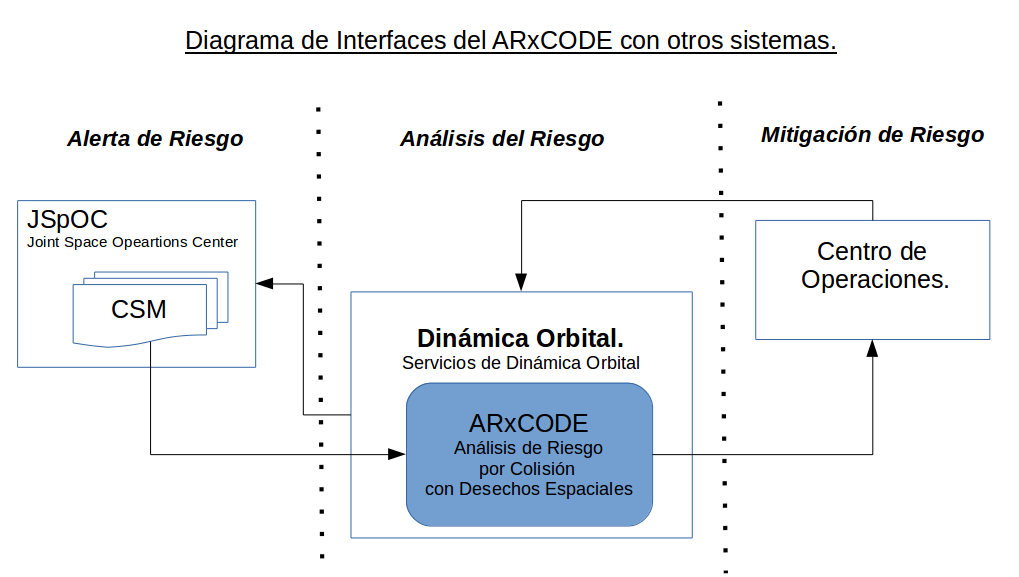
\includegraphics[width=0.8\textwidth]{imagenes/interfasessistemas}}
  \caption[Diagrama de Interfaces del Sistema]{Diagrama de Interfaces del Sistema}
  \label{fig:interfaces}
\end{figure}

No obstante, por cuestiones de tiempo y de accesibilidad, para el desarrollo de este trabajo, los datos que provee el departamento de din\'amica orbital fueron descargados y se extraen de un directorio, al igual que los mensajes de alerta CDM, que fueron descargados de pa\'aginas de internet , ya que no nos han facilitado ninguno vinculado a la misi\'on operativa de la que cual procesamos los productos orbitales, por motivos de confidencialidad. Se realiz\'o la automatizaci\'on de la descarga de TLEs de la p\'agina Space-Track y se habilit\'o en la interfaz la pantalla que permite la carga manual de los datos del encuentro.\\

En conclusi\'on, las interfaces implementadas, son (Ver Fig. \ref{fig:interfacesImpl}):\\
\begin{itemize}
\itemsep0em
 \item Conexi\'on a Space-Track para la solicitud de TLEs.
 \item Administraci\'on de las efem\'erides orbitales de los directorios de CodsAdmin.
 \item Administraci\'on de los CDM del directorio CDM, a trav\'es de la intervenci\'on del operador.
 \item Carga Manual de datos de un encuentro realizada por el operador.
\end{itemize}

\begin{figure}
\centering
  \fbox{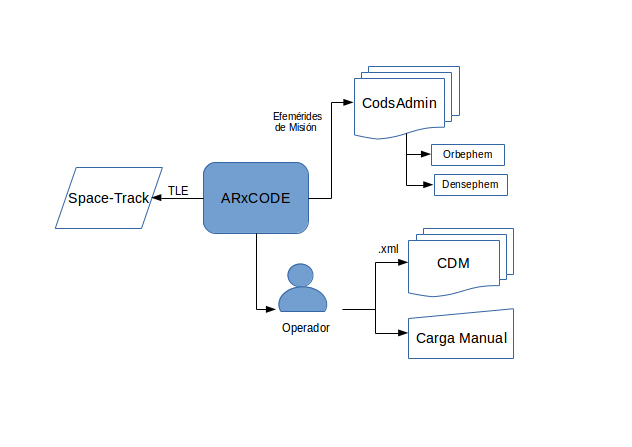
\includegraphics[width=0.8\textwidth]{imagenes/interfazImplementada}}
  \caption[Diagrama de Interfaces Implementadas en ARxCODE]{Diagrama de Interfaces Implementadas en ARxCODE}
  \label{fig:interfacesImpl}
\end{figure}

\section{Arquitectura}


\subsection*{Componentes}\label{subsec:componentes}
En un planteo conceptual, con alto grado de abstracci\'on, los distintos paquetes de ARxCODE pueden agruparse en cinco componentes Fig.  \ref{fig:componentes}: PROCESAMIENTO, ADMINISTRACI\'ON DE DATOS, INTERFAZ GR\'AFICA Y VISUALIZACI\'ON, Sistemas de Referencia y VALIDACIONES.\\

\begin{itemize}
 \item PROCESAMIENTO: Involucra los cuatro paquetes que no s\'olo operan con los datos ingresados, sino que tambi\'en los manipulan y procesan para generar nuevos productos. Estos m\'odulos son, de alguna manera los distintos n\'ucleos del c\'odigo.\\
 \begin{itemize}
 \itemsep0em
  \item {\it{AjustarTle}}
  \item {\it{Comparar}}
  \item {\it{Estadistica}}
  \item {\it{Encuentro}}
 \end{itemize}
 \item ADMINISTRACI\'ON DE DATOS: Son aquellos paquetes que se encargan de la obtenci\'on, el desgloce y el preprocesamiento de los datos que ser\'an utilizados por el resto de los m\'odulos.
 \begin{itemize}
 \itemsep0em
  \item {\it{TleAdmin}}
  \item {\it{CodsAdmin}}
  \item {\it{CDM}}
 \end{itemize}
 \item INTERFAZ Y VISUALIZACI\'ON: Agrupa el paquete que genera la interfaz gr\'afica y el paquete que contiene todos los m\'odulos que generan represntaciones visuales, como los ploteos o los tracks de las trayectorias de los objetos.\\
 \begin{itemize}
 \itemsep0em
 \item {\it{Aplicacion}}
 \item {\it{visual}}
 \end{itemize}
 \item Sistemas de Referencia: {\it{SistReferencia}}, es el paquete que contiene todo lo referente a las transformaciones entre los distintos sistemas de referencia, ya sean espaciales o de tiempo.
 \item VALIDACIONES: Agrupa todos los m\'odulos desarrollados para validar los resultados.
\end{itemize}


\begin{figure}[h!]
  \centering
  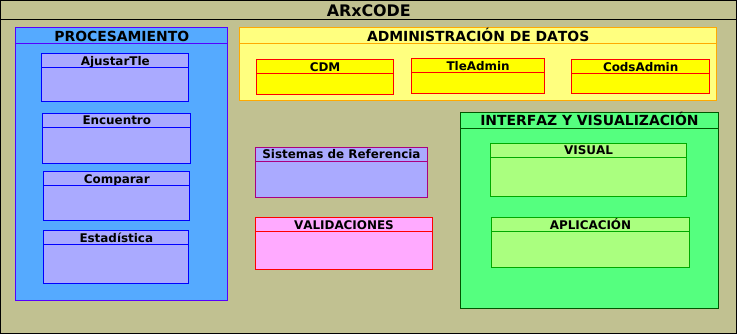
\includegraphics[width=.8\textwidth]{imagenes/componentesAR}
  \label{fig:componentes}
  \caption{Componentes de ARxCODE}
\end{figure}


\subsection{Casos de Uso}

Este trabajo se pens\'o como un adicional, o un \textcolor{red}{agregado}, al software principal del departamento de din\'amica orbital. En este sentdio, no existe gran complejidad en la estrucutura del prototipo, ya que su valor, radica en la correcta implementaci\'on de los algoritmos que procesan la informaci\'on del encuentro.\\
Identificamos dos clases de uso Fig. \ref{fig:casosuso} :\\
\begin{itemize}
 \item {\it{Procesar Encuentro}}: que nuclea el procesamiento vertebral de ARxCODE
 \item {\it{Ver informes de encuentros anteriores}}: ofrece encuentros anteriores.
\end{itemize}

\begin{figure}[h!]
  \centering
  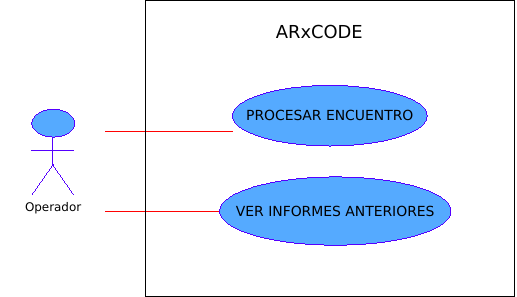
\includegraphics[width=.5\textwidth]{imagenes/usecaseAR}
  \label{fig:casosuso}
  \caption{Casos de Uso de ARxCODE}
\end{figure}


 \begin{table}[h]
\centering
\resizebox{18cm}{!}{
\begin{tabular}[c]{|l|l|}
\hline
\bf{Nombre}  &    \it{Procesar Encuentro}\\
\hline
Actor  &    Operador de Din\'amica Orbital con Autorizaci\'on\\
\hline
\multirow{ 3}{*}{Prop\'osito} & Calcular la probabilidad de colisi\'on, la m\'inima distancia total\\
& y m\'inima distancia en la coordenada radial, para poder hacer un an\'alisis\\
& de la situaci\'on de encuentro.\\
\hline
\multirow{ 4}{*}{Resumen}& Procesa la ingesta de datos de un encuentro, (CDMs o ingreso manual)\\
&  y calcula los par\'ametros de la situaci\'on de riesgo:\\
& m\'inima distancia total, m\'inima distancia en la coordenada radial y probabilidad de colisi\'on.\\
& Realiza gr\'aficos e informes.\\
\hline
Requerimientos  &    \\
\hline
\multirow{ 3}{*}{Precondiciones}  &  El operador debe estar registrado en la p\'agina space-track de NORAD.  \\
& Los archivos CDM deben estar previamente cargados en el Directorio de b\'usqueda.\\
& El operador debe conocer el encuentro que desea analizar y sus datos en caso del ingreso manual.\\
\hline
\multirow{ 3}{*}{Flujo Principal} & 1 - El operador selecciona un archivo CDM \\
& 2 - El operador oprime el bot\'on {\it{Track}} para visualizar el encuentro proyectado en la superficie terrestre (opcional)\\
& 3 - El operador oprime el bot\'on para genera un informe (opcional)\\
\hline
\multirow{ 3}{*}{Flujo Alternativo} & 1 - El operador ingresa los n\'umeros de identificaci\'on de los objetos (NORAD\_ID) \\
& 2 - El operador ingresa la fecha y hora del m\'aximo acercamiento (TCA)\\
& 3 - El operador oprime el bot\'on {\it{Procesar}} para procesar el encuentro\\
\hline
Postcondiciones & El informe de an\'alisis de riesgo fue generado y almacenado.\\
\hline
\end{tabular}}
\caption[Caso de Uso: Procesar Encuentro]{Tabla con la descripci\'on del caso de uso: \it{Procesar Encuentro}}
\label{tab:usoproceso}
\end{table}

\begin{figure}[h!]
  \centering
  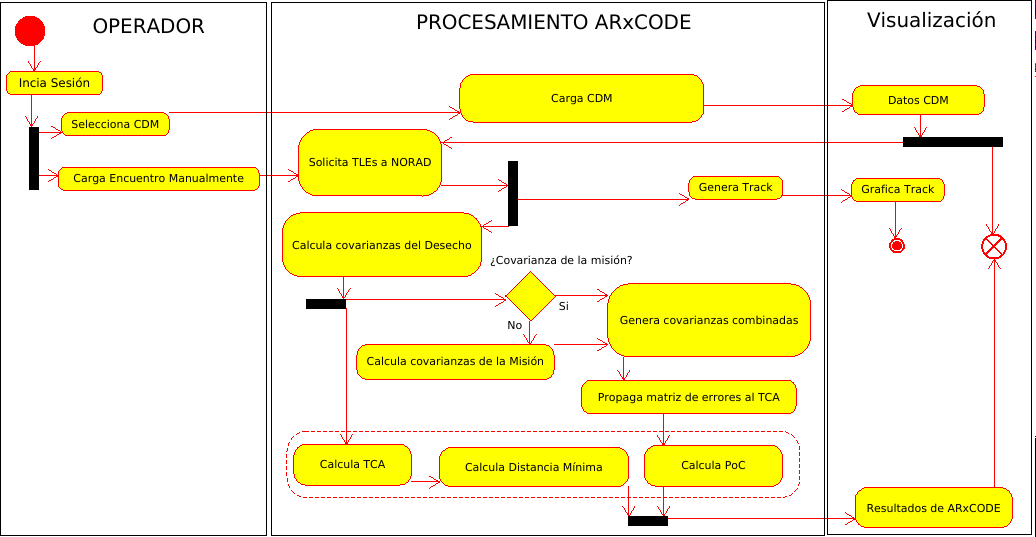
\includegraphics[width=\textwidth]{imagenes/actdiagAR}
  \label{fig:actdiag}
  \caption{Diagrama de Actividades de ARxCODE}
\end{figure}

\section{Entradas y Salidas}

archivos y demases

\subsection*{Preprocesamiento de los Datos de Misi\'on de CODS}
Para este trabajo CONAE nos facilit\'o el acceso a los datos orbitales de la misi\'on SAC-D.
Los datos se ecuentran montados en un servidor que contiene la informaci\'on organizada en archivos con formato ASCII, distribuidos en distintas carpetas seg\'un su clasificaci\'on.\\
Para la comparaci\'on que proponemos, solicitamos acceso a los archivos de efem\'erides orbitales ORBEPHEM, que ofrecen posiciones y velocidades tabuladas cada un minuto, en el Sistema de Referencia TOD (True of Date), en coordenadas cartesianas.

\subsection*{ORBEPHEM}
Estos productos son generados luego de un post procesamiento que incluye una propagaci\'on ajustada por una determinaci\'on orbital. 
Cada archivo contiene un listado cronol\'ogicamente tabulado de posiciones y velocidades, dentro de un periodo de casi 3 d\'ias. ( doc\_interfaces)

La nomenclatura de los mismos respeta el siguiente formato:\\
\begin{verbatim}
 CODS_YYYYMMDD_HHMMSS_SACD_ORBEPHEM_TOD_XYZ_O.TXT
 
 Donde:
  CODS = Identifica el Servicio dentro del CUSS que presta la información.
  YYYYMMDD_HHMMSS = epoca de generación del dato.
  SACD = Identificación del Satélite.
  ORBEPHEM = Tipo de Dato, Efeméride Orbital (procesada a posteriori)
  TOD = Sistema de Referencia True of Date.
  XYZ = Tipo de efeméride, cartesiana.
  O = Operacional. 
\end{verbatim}


\subsection*{Archivos Utilizados}
Si bien la nomenclatura de los archivos respeta una estructura, s\'olo se indica en el nombre, la fecha de generaci\'on de los datos y no puede desprenderse del mismo cu\'al es la \'epoca final e inicial de cada archivo, y no existe un registro del los gaps de datos ausentes. A su vez, las \'epocas contempladas en cada uno de ellos no está homogeneizada. Es decir, la fecha y hora inicial y final de cada registro es diferente para cada archivo.\\
Dada esta organizaci\'on, para el punto tres del procedimiento, referente a la localizaci\'on del archivo necesario para la comparaci\'on, la b\'usqueda se realiza de la siguiente manera:\\
Localizamos en primer lugar el archivo cuyo nombre coincide con la fecha de la \'epoca del TLE primario.
Como una misma fecha se encuentra en m\'as de un archivo, buscamos el archivo que contenga esa fecha y que adem\'as sea el m\'as actualizado de todos. Para ello, además del archivo cuyo nombre contiene la fecha del TLE primario, se enlistan los siguientes dos archivos y se ordenan en orden decreciente, de manera que el primer lugar de la lista lo ocupe el \'ultimo de los archivos seleccionados. Finalmente se comienza el proceso iterativo de abrir los archivos, evaluar el contenido y ver si se encuentran los dos registros que encierren la \'epoca del TLE.
Una vez que se encuentran las l\'ineas de efem\'erides que contienen la \'epoca de inter\'es se interpola, y se termina la iteraci\'on.

\noindent
Cantidad TOTAL de archivos $=  1454$\\
Cantidad media de resgistros por archivo $=  2688$\\
Archivo con el mayor n\'umero de registros $=  3042$\\
Archivo con el menor n\'umero de registros $=  142$\\


\section*{Diferencias}

\begin{itemize}
 \item Revisar escritura sobre datos CODS.
 \item Comparar defasaje inicial con defasaje de TLE respecto de GPS. (ver tendencias - empezar a diagramar los apédices)
 \item Comparar errores lineal vs cuadr\'atico.
\end{itemize}
